\chapter{Theoretical Background}

This chapter introduces the fundamental concepts such as the \textit{cost estimation process}, a \textit{state-of-the-art report}, different \textit{estimation methods} and \textit{techniques}. The cost estimation process in IT projects and the different methods to calculate the cost of a project are described in this chapter. The \textit{state of the art} report combined with the \textit{market description} will give a short overview over the situation about software estimation tools on the market and the possibility of a \textit{mobile solution} for cost estimations. \textit{Android} as the chosen platform and \textit{Java} as the programming language will not be described in detail here and are assumed to be known.

\section{Cost estimation in software engineering}

One of the most expensive components of computer systems are software products. While private clients are mostly interested in the final price of a product, business clients of IT companies typically want to know the \textit{costs} of the software \textbf{before} project launch. As analyzed in the \textit{IT-Trends} study from \textit{Capgemini} \cite{capgemini} the IT budget of companies is growing up to 10\% every year. Whether developing a new project or standardizing existing software, minimizing the project costs is always a \textit{main goal} of the project management. As human resources are the biggest part of software costs, project managers and especially business clients want to know the estimated spendings and completion time of a project, which derives the needed manpower. Most of the estimation methods focus on this aspect and give the result in \textit{man days}. These estimated days can then be converted into the real costs by calculating the daily rate with the estimated time.
\\
Basically the cost estimation in software engineering wants to answer the following questions:
\begin{enumerate}
\item How much effort is required to complete the project?
\item How much days are needed to complete the project?
\item What is the total cost of the project?
\end{enumerate}
While projects are a living thing, the effort may change due to unexpected difficulties. For a precise estimation of the total costs, an adjustment cannot be avoided and it can be useful to change the estimation method in a later project phase. This means that the estimation process is not an \textit{one-time} thing but will change through the life-time of a project \cite{itplanung}. 


\subsection{Estimation Process}

It is common to create the first cost estimation before the system design, but also for monitoring purposes, milestones or if the client wants an overview of the project. Each time an actual cost estimation is needed the estimation process is executed which is a set of techniques and procedures that are used to derive the software cost estimate. Kathleen Peters described the basic process of an estimation, as seen in figure \ref{fig:basicEstimationProcess}, as it is common in the industry \cite{estimationProcess}. As can be seen in the figure, there are seven steps in this estimation process. The first part is to collect the \textit{initial requirements} which is essential to know what the project is about and evaluate the approximate project size. With a selected estimation method, which is described in section \ref{chapter:estimationmethods}, the evaluated size of the project is then estimated. Afterwards the effort in man days is calculated, from which the cost schedule is created. Data from older projects can be included into the cost estimation which allows a more precise estimation. In the process step to \textit{approve the estimation}, it has to be decided if the costs are acceptable or if the range of functions has to be shortened and the re-estimation has to be started from the beginning. If the cost estimation is acceptable the development of the product can start or continue.\\
\begin{figure}[h] 
	\centering 
	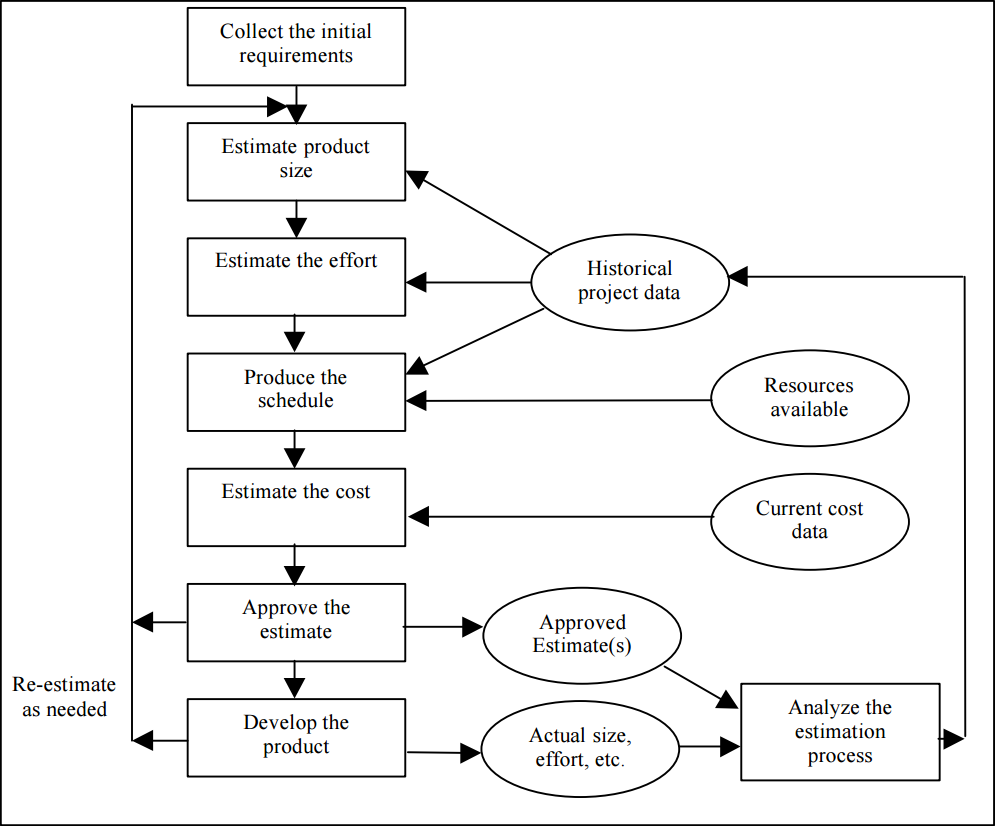
\includegraphics[width=13cm]{images/estimationProcess.PNG} 
	\caption{- The Basic Project Estimation Process}
	Source: Peters, Kathleen - Software Project Estimation, Page 3  
	\label{fig:basicEstimationProcess}
\end{figure}\\
In this classical view of the estimation process there are four outputs generated:
\begin{enumerate}
	\item \textit{Actual Size} - the size of the project as a numerical value to make it comparable.
	\item \textit{Manpower Loading} - the amount of personnel that is allocated to the project.
	\item \textit{Project Duration} - the time that is needed to complete the project.
	\item \textit{Effort} - the amount of effort required to complete the project is usually measured in units as man days (MD) or person months (PM).
\end{enumerate}
As described before, the estimation process can be triggered at any time in the project to re-estimate the costs. Depending on the project stage another estimation method than used in the stage before can be more precise.\\
The overview in fig. \ref{fig:estimationMethodInStage} shows that the \textit{SLIM} method is more suitable at the beginning of a project, whereas the \textit{ZKP} method is more suitable after the system design stage\footnote{\url{http://winfwiki.wi-fom.de/index.php/Methoden_und_Verfahren_der_Aufwandsch\%C3\%A4tzung_im_Vergleich}}. Most of the estimation methods are useful after the \textit{'Study'} stage. This is because a rough overview of the project size exists afterwards. Different estimation methods may also change the \textit{evaluation output}, which is one of the difficulties of cost estimations.\\
\begin{figure}[h] 
	\centering 
	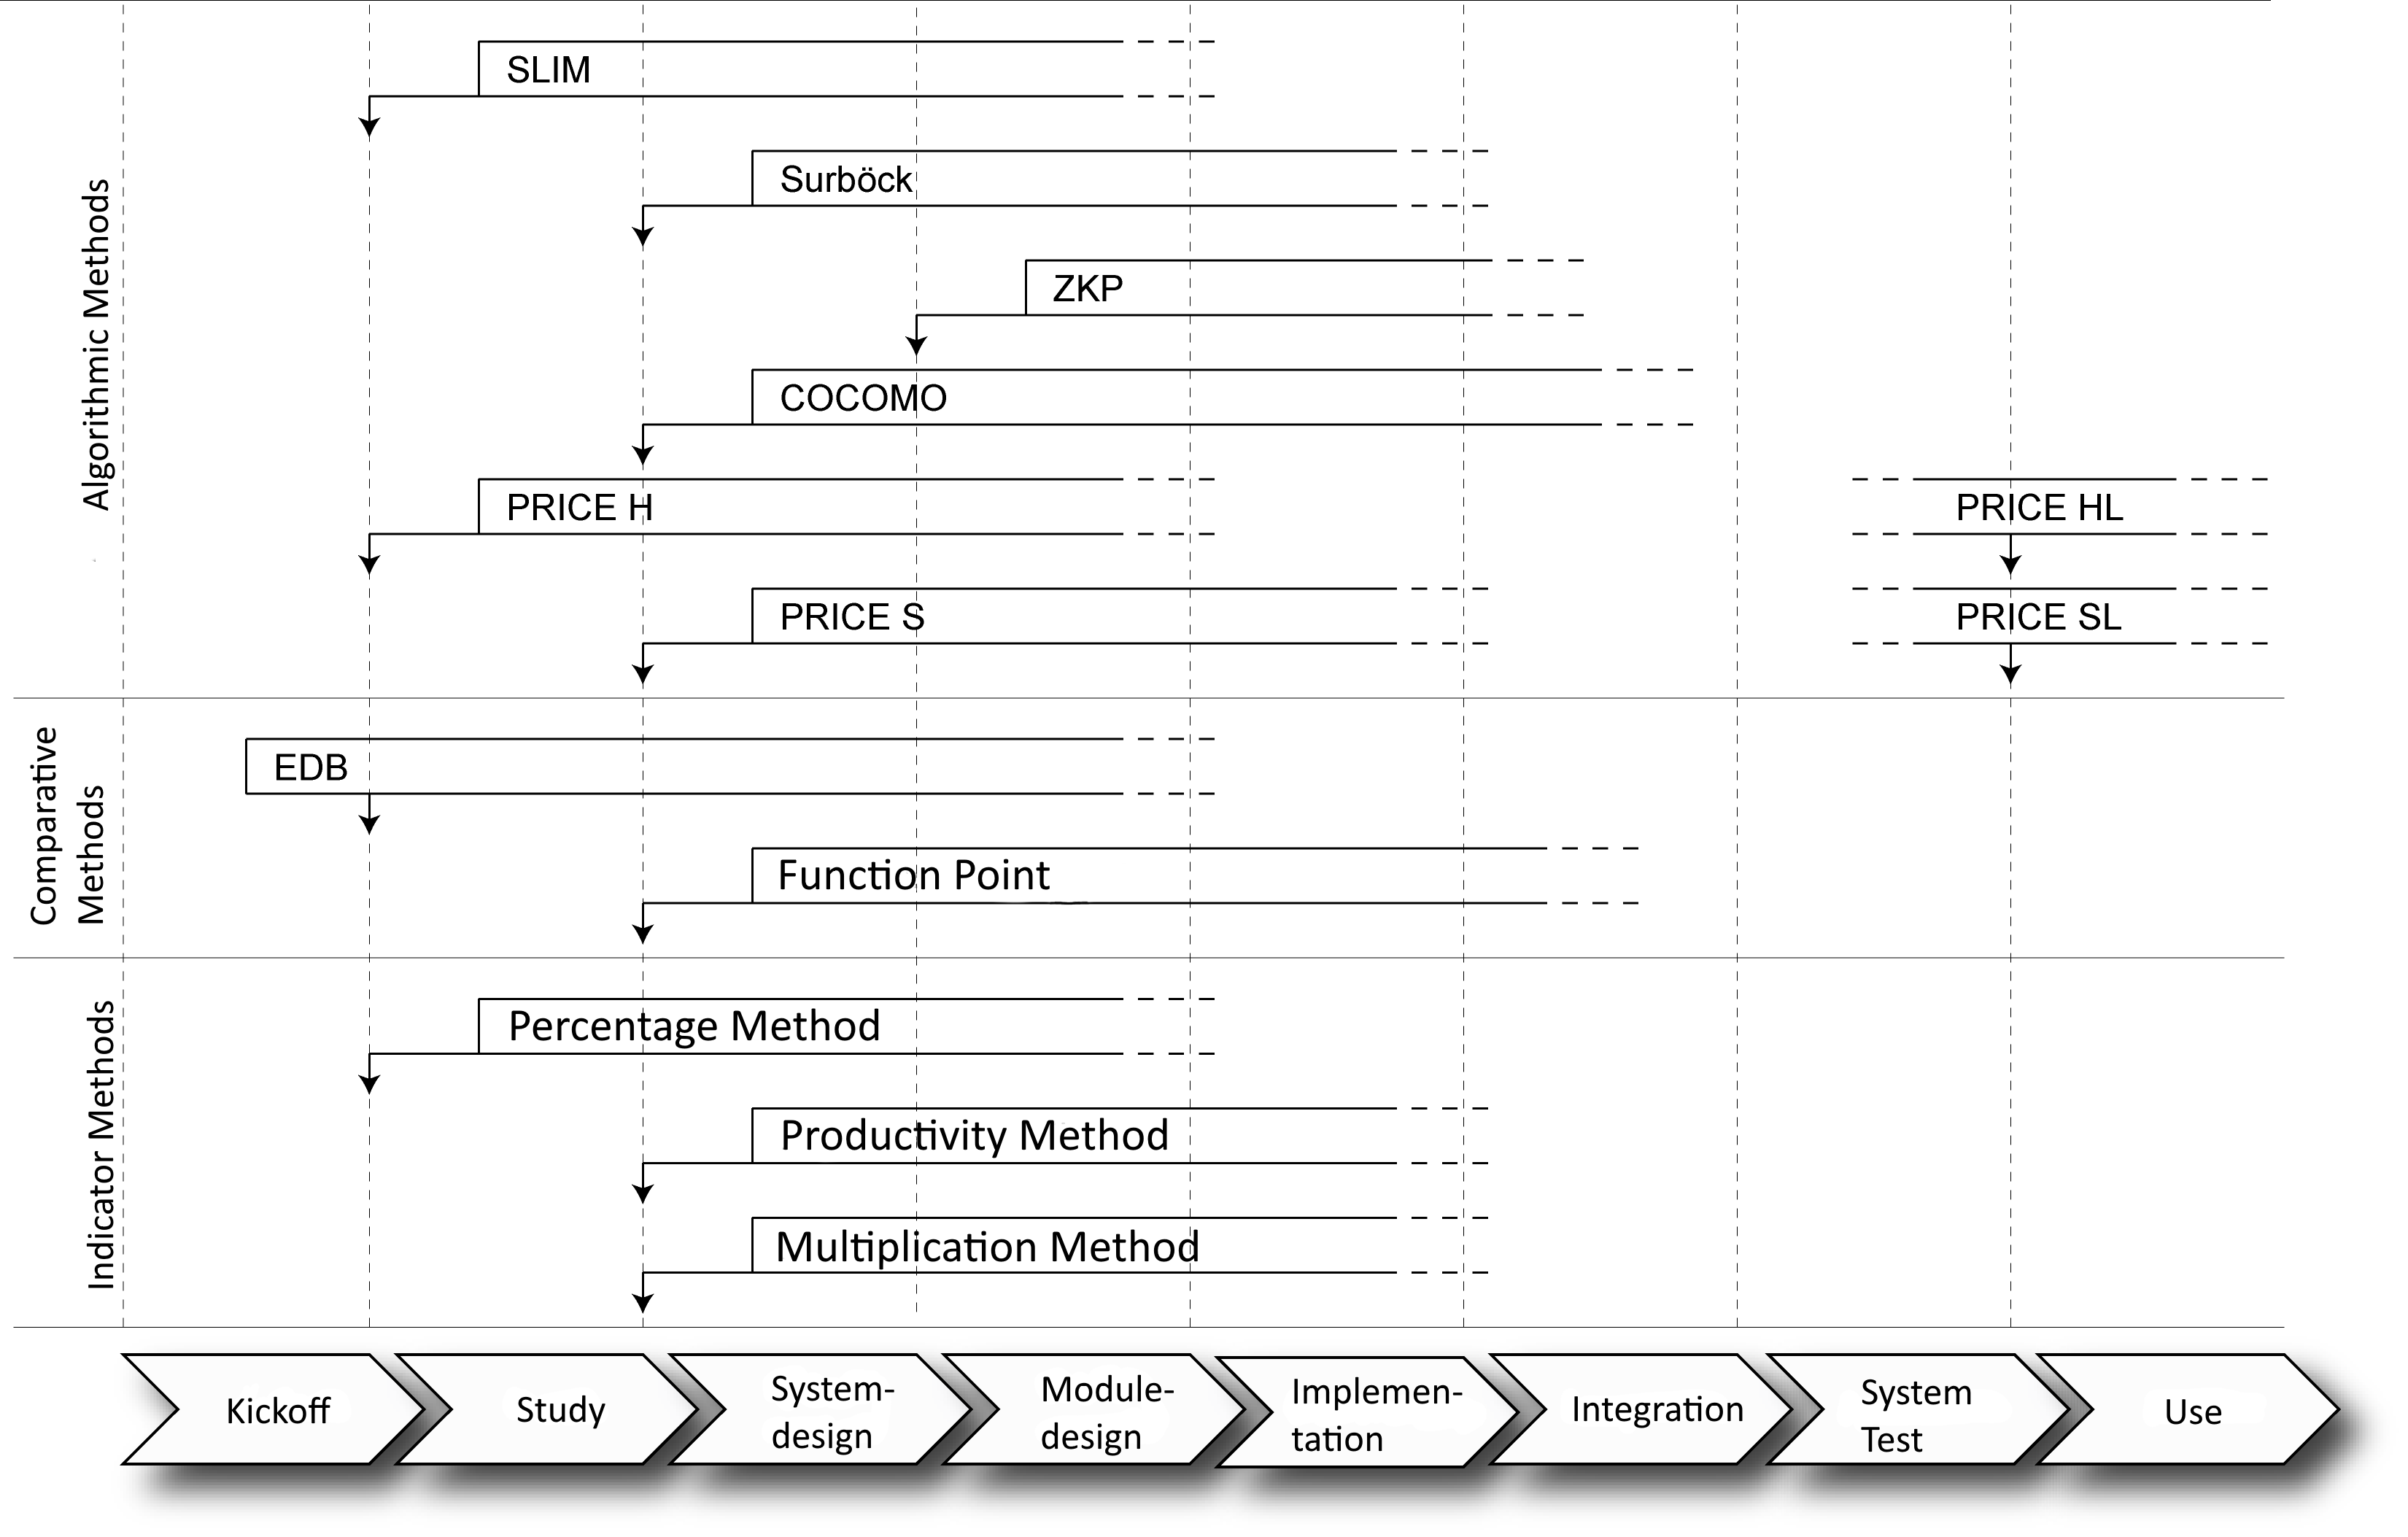
\includegraphics[width=13cm]{images/Einsatzzeitpunkte2.PNG} 
	\caption{- Starting Points of Estimation Methods} 
	\label{fig:estimationMethodInStage}
\end{figure}

\subsection{Difficulty of estimations}

One of the problems in estimating costs is that the actual code is only a small part of the project. Beside project planning there are many administrative tasks to do, like coordination of the project or searching and fixing errors. Most estimation methods evaluate the estimated time for the implementation only and too little or no time is evaluated for the non implementation tasks. This resolves in an underestimation of the non implementation tasks or an overestimation, if they are predicted as a high value \cite{itplanung}.
\\
Most project managers rely on their experience from past projects. This is an advantage, but as technology changes fast and new projects inherit new problems, there is no prior experience for some parts of it, which is another estimation difficulty. This can make experiences from prior projects useless. Because of the unique nature of projects it is common that a new project has big parts where no experience exists. Another difficulty of estimations is the fact that people who are inherited have a more positive outlook and mostly underestimate the costs.
Also, customers often got a target time for the project, which leads in adjustment of the cost estimation. This leads to budget overrun if the needed resources are not available for the project \cite{winfwiki}. It is also not guaranteed that the estimated costs are accurate and stay within the budget. An estimation can easily go past their estimated target as new technologies and unexpected difficulties are commonplace. A partial requirements engineering can also cause an inaccurate cost estimation due to unexpected difficulties in the implementation.\\

\subsection{Methods for estimation}\label{chapter:estimationmethods}

Estimation methods are different metrics to calculate the costs of a project and there are different approaches to categorize the estimation methods. The categorization used in this paper is based on the book \textit{'Management von IT-Projekten'} by Hans W. Wieczorrek, where the methods are subdivided in \textit{algorithmic}, \textit{comparative}, \textit{key figures} and \textit{expert discussion} method\cite{itplanung}.\\
All estimation techniques have in common, that only with a combined use of these different estimation methods a suitable result can be achieved as a measured value for the project. For the evaluation of the needed effort the underlying metric describes how this calculation is done. On the basis of charge rates, the effort size is calculated out of it.\\

\subsubsection{Algorithmic Method}

The algorithmic method uses a closed formula, which is based on empiric evaluation of already terminated projects or on existing mathematically models. Different forms of this method are the weight and the sampling method, which only differ in their usage.\\
The accuracy of the estimation depends primarily on the precision of the influence factors \cite{itplanung}. The algorithmic method always connects measurable project sizes, such as \textit{lines of code} and \textit{implementable features}, with influencing factors to get the result, represented as required effort in personnel costs. The basic formula for this method, as described by Wieczorrek \cite{itplanung} is:

\begin{equation}
	Personnel costs = f(result quantity, influencing factors)
\end{equation}

\subsubsection{Comparative Method}

Not based on a formula or numerical connection, the comparative method tries to create a reference between the current project and past projects. Therefore projects from the own company or the same industry sector are analyzed with appropriate comparison methods. This estimation method has the advantage, that it can be used early in project development \cite{itplanung}. This method can be used for hardware and software projects.

\subsubsection{Key Figures Method}

Estimation methods based on key figures can be separated into a \textit{multiplication} and a \textit{percentage} method. The \textit{multiplication} method uses units of power as the base to estimate the total expenditure, whereas the \textit{percentage} method uses the effort of a project stage to estimate the effort for the next stage.\\
After project completion, a post calculation determines the total project costs and the amount of specific types of costs. In order to calculate these costs, they will be divided by the scope of the developed product. This results in new key figures which can be used for new projects by multiplication of the estimated scope with the appropriate key figures. Regular updates of the key figures is necessary for the right results \cite{itplanung}.\\

\subsubsection{Expert Discussion Method}

As a quantitative and heuristic method the expert discussion uses knowledge from selected groups of people. It differentiates between four kinds: \textit{single person interview}, \textit{multiple person interview}, \textit{Delphi method} and \textit{assessment meeting}.\\
The advantage of this estimation method is that they are useful for all project types. But they have the risk of a strong affection by subjective opinions and the experience of the interviewees. As a result, expert discussions should never be used for complete projects, only for sub projects \cite{itplanung}.\\

\section{Estimation Techniques}

The existing estimation techniques rely on experience-based judgments by project managers
who created, by combining estimation methods, techniques that can be used to estimate the effort of a project. Most of the estimation techniques became popular in the 80's. With the agile projects becoming more popular, estimation techniques for these project types are also rising. \\
Because of the fundamental uniqueness of the projects nature, an \textit{'universal, everywhere applicable and always delivering the correct estimation'} technique does not exist, according to Litke \cite{litke}. There is also no clear selection progress for the estimation technique to use, beside the time aspect, when the use of a technique is available. As shown in figure \ref{fig:estimationMethodInStage}, the \textit{Function Point} and the COCOMO technique are both possible after the study stage. As a comparative method, the function point technique has not much in common with COCOMO, which is an algorithmic technique. The project manager has to balance the weigh of each technique and probably choose the one he has the most experience with. As an example for estimation techniques these will be described here in more detail and a comparison at the end of this chapter.


\subsection{Function Point} \label{FPMethod}

The Function Point technique was first mentioned by Allan J. Albrecht in 1979 at the IBM symposium \cite{albrecht}. He declared that an useful measurement of productivity is only possible in relation to the functionality that is visible to the user. This measured productivity needs to be independent of the used technology and is calculated with the proportion of project effort and the allocated function points.\\
This resulted in the idea to turn over this calculation for a preliminary estimation of the effort the project would have. Because of the clarity and the flexibility, the technique spread fast. \\
It helps to estimate the scope of a project to an early stage and is suitable for benchmarking in the own company as well as on a national or international level \cite{FPKompakt}. It contains algorithmic and also comparative methods. Basically, this technique uses five steps for estimation \cite{jenny}:
\begin{enumerate}
	\item Determining the components
	\item Evaluation the components
	\item Calculating the function points
	\item Categorization the influence factors
	\item Calculating the development effort with the function points and influence factors
\end{enumerate}
The most important part of this technique is, that all measurements only include the user view. This means that the user view focuses on the functions that are important for the specific business process. Implemented business processes are the components that have to be determined.

\subsubsection{Determining the Components}\label{fpcomponents}

To divide the project in useful components, all inherited business processes are divided into an elementary process.This distinction is made into five categories:
\begin{enumerate}
	\item Input Data
	\item Output Data
	\item Request
	\item Dataset
	\item Reference Data
\end{enumerate}
The \textit{Input Data}, sometimes called \textit{External Inputs} (EI), is an elementary process in which data crosses the boundary from the outside of the application to the inside. This data comes from a data input screen or another application. Maintaining one or more logical files it is used to control business informations.\\
\textit{External Outputs} (EO), or \textit{Output Data}, are an elementary process in which derived data passes across the boundary from the inside to the outside. Created output files or reports are sent to other applications. These are created from one or more internal logical files and external interface files.\\
Internal \textit{Logical Files} (ILF’s) or \textit{Dataset} are an user identifiable group of logically related data that resides entirely within the applications boundary and is maintained through external inputs.\\
The next category are \textit{Requests} or \textit{External Inquiry} (EQ). An elementary process with both input and output components that result in data retrieval from one or more internal logical files and external interface files. This process does not update any \textit{Internal Logical Files}, and the output side does not contain derived data.\\
The last category is the \textit{Reference Data} or \textit{External Interface Files} (EIF), which are a user identifiable group of logical related data that is used for reference purposes only. This data resides entirely outside of the application and is maintained by another application \cite{fpafundamentals}.\\
These are the smallest and from a business perspective most useful and closed activities, that can be performed by the system \cite{FPKompakt}. It is useful to categorize the components, because a change in the datasets is followed by more effort than changing a request \cite{itplanung}. After the categorization there is an amount of items for each category which has then to be evaluated in the next step.

\subsubsection{Evaluation the Components}

The evaluation of the components is the classification of each category in their level of difficulty (simple, medium or complex). After this, each component is multiplied with the point value according to their difficulty. The table \ref{tab:pointvalues} is described by Wieczorrek and are standard values for the function point technique \cite{fpafundamentals}.

\subsubsection{ Calculating the amount of Function-Points}

After the evaluation there is an amount of components for each category. To get the number of function points each category has to be multiplied according to the selected weigh and all categories are summed up. This results in the equation \ref{fp:E1}.\textit{Function} is the respective category and the \textit{Difficulty} is the weigh from table \ref{tab:pointvalues}. The resulted value \textit{E1} is necessary for evaluating the estimated points with the influence factor.
\begin{equation}
	\textit{E1} =  \sum \limits_{1}^n  (\textit{Function} \cdot \textit{Difficulty}) \label{fp:E1}
\end{equation}
\begin{table}[h] 
	\centering 
	\setlength{\tabcolsep}{4pt}
	\begin{tabular}{|l|c|c|c|}\hline
		Category & simple & medium & complex \\ \hline
		Input Data & 3 & 4 & 6\\ \hline
		Output Data & 4 & 5 & 7\\ \hline
		Request & 3 & 4 & 6\\ \hline
		Dataset & 7 & 10 & 15\\ \hline
		Reference Data & 5 & 7 & 10\\ \hline
	\end{tabular}
	\caption{Point value of each category} 
	\label{tab:pointvalues} 
\end{table}
\subsubsection{ Classification the Influence Factors}\label{fp:classificationInfluence}

To get a more realistic estimation, all influences that can affect the projects surroundings are measured. There are seven defined influence factors \cite{Softwaremanagement}, which are described below. Each of the influence factors has a value between zero and five which describes how much the factor influences the project. Exception are \textit{Arithmetic Operation} and \textit{Exception Regulation} which go from \textit{zero} to {ten}.\\

\begin{enumerate}
	\item \textbf{Integration into other applications}\\This factor describes if the system will work with the distributed data. Zero means that the system does not work with other applications and five means that there is an integration into other applications in both ways, sending data to other applications and receiving data.
	\item \textbf{Local Data Processing}\\The system will work with different applications and will send and receive data from other applications. This shows whether there is a cooperation with other applications and if the communication exists online or offline.
	\item \textbf{Transaction Rate}\\A high transaction rate affects planing, development, installation and maintenance of the system. It describes how much transactions are expected within the system.
	\item \textbf{Processing Logic}\\The processing logic is divided into 4 subcategories: \textit{Arithmetic Operation}, \textit{Control Procedure}, \textit{Exception Regulation} and \textit{Logic}. \textit{Arithmetic Operation} describes the intensity of the operations in the project. The controlling of the results is stated within the \textit{Control Procedure}. The \textit{Exception Regulation} describes how eventual exceptions are treated and the \textit{Logic} multiplier describes how much effort is to be expected for planning the logical component of the project.
	\item \textbf{Reusability}\\ How much of the produced software has to be reusable in other projects is described with this category? A high value means extra effort in the planning stage for module-based development.
	\item \textbf{Stock Conversion}\\ This describes how much of the data needs to be transformed for the usage within the project. A high value means, that a lot of input data from other applications have to be transformed into data the application can process.
	\item \textbf{Facilitate Change}\\ The application was especially planned and developed in such a way that changes can be made easily. A high value means that the user can make changes on the system on their own and that the changes are available immediately.
\end{enumerate}
When all influence factors are set, all values for each factor will be summed up to the value \textit{E2}, as described in the following equation. 
\begin{equation}
\textit{E2} =  \sum \limits_{1}^n   \textit{Influence Factor}  \label{fp:E2}
\end{equation}\\
This influence factor indicator then has to be transformed into a multiplier that calculable with function points \cite{Softwaremanagement}\cite{fpafundamentals}.  

\begin{equation}
	\textit{E3} =\frac{\textit{E2}}{100}  + 0,7 \label{fp:E3}
\end{equation}

\subsubsection{Calculation the Function Points}

With the calculated Function Points (\textit{E1}) and the Influence Factor multiplier (\textit{E3}) the \textit{total-function-points} (TFP) can now be calculated with the following formula:
%equation,formula
\begin{equation}
	\textit{TFP} = \textit{E1} \cdot \textit{E3}  \label{fp:TFP}
\end{equation}\\
These \textit{TFP} have no unit and represent only points. They have to be calculated into man days with a \textit{points-per-day} value. From the regression analysis of previous projects a standard calculation of Function Points per day can be made using table \ref{tab:pointsperday}.\\
The project has to be classified with their Total-Function-Points and divided through the appropriate points per day, as described in \ref{tab:pointsperday}. This results in the expected man days for this project.\\
\begin{table}[h] 
	\centering 
	\setlength{\tabcolsep}{4pt}
	\begin{tabular}{|l|c|c|}\hline
		Estimated Size    & Function Points & Points per Day\\ \hline
		Small Project     & $\le$350        & 18 \\ \hline
		Mid Small Project & $\le$650        & 16 \\ \hline
		Medium Project    & $\le$1100 		& 14 \\ \hline
		Mid Large Project & $\le$2000 		& 12\\ \hline
		Large Project     & $\ge$2000 		& 10 \\ \hline
	\end{tabular}
	\caption{Function Points to Days} 
	\label{tab:pointsperday} 
\end{table} 

\subsection{COCOMO} \label{COCOMOMethod}

The Constructive Cost Model (COCOMO) is mostly used when it's not possible to rely on experience. It is based on algorithmic and parametric methods that merge parameters from \textit{software projects}, combining the \textit{system size}, \textit{product properties}, \textit{project} and \textit{team factors} with the \textit{effort for developing} the system \cite{jenny}.\\
As a public domain model it is free to use and is considered to be a classic for algorithmic methods. This technique was adjusted to the IT development through the years and is common in many companies.
The accuracy of the COCOMO techniques rises with later project stages. The deviation of the cost estimation at the beginning of the project is between \textit{0,25 $\cdot$ MD} and \textit{4 $\cdot$ MD}. In later project stages this variation decrease until it is zero just before the project ending \cite{sommerville}.\\
The parameters for COCOMO can be split into three parts. The \textit{project classes}, \textit{model variants} and the \textit{implementation time and effort}.

\subsubsection{Project Classes}

The \textit{project classes} represent the estimated size of the program itself. These are expressed in \textit{kilo delivered source instructions} (KDSI). COCOMO classifies three project classes with different calculation factors as described in table \ref{tab:projectclasses} \cite{sommerville}.

\begin{table}[h]
	\centering 
	\setlength{\tabcolsep}{4pt}
	\begin{tabular}{|l|c|c|p{6cm}|}\hline
		Complexity	& Calculation Factor& KDSI 	& Describtion\\ \hline
		Small   	& 1.05        		& $<$ 50  			& A small, well-known project team works together, the environment is well-known, there is no big innovation necessary and no pressure due to a deadline.\\ \hline
		Medium 		& 1.12        		& 50 - 300 			& Employees with average experience, team members with some experiences in different parts of the project are working together.  \\ \hline
		Complex 	& 1.20 				& $>$ 300 			& High cost and deadline pressure, high innovations and an extensive project. High requirements to the project team and new components.  \\ \hline
	\end{tabular} 
	\caption{COCOMO project classes} 
	\label{tab:projectclasses} 
\end{table}

\subsubsection{Model Variants}

The COCOMO technique can be differed into a \textit{basis}, \textit{intermediate} and \textit{detailed model}. These represent the detail level of the cost estimation.\\
The first stage is also called \textit{basis estimation} and is a rough estimation, which estimates the project costs to an early stage of the project. The costs are calculated with an equation without dividing the project into structure or time aspects. The base model is an useful starting point for later estimations.\\
The second stage is the \textit{intermediate} model and adjusts the first estimation to a higher level of detail by differentiating the development stages. It is not a parametric estimation yet, because not all data can be considered.\\
The \textit{detailed model} is the last stage of the estimation and allocates the estimation with fifteen influence factors \cite{jenny}. These influence factors are divided into four categories.
\begin{enumerate}
	\item \textbf{Product Attributes}
	\begin{enumerate}
		\item Required Software Reliability
		\item Size of the Application Database
		\item Complexity of the Product
	\end{enumerate}
	\item \textbf{Hardware Attributes}
	\begin{enumerate}
		\item Run-time Performance Constraints
		\item Memory Constraints
		\item Volatility of the Virtual Machine Environment 
		\item Required Turnabout Times
	\end{enumerate}
	\item \textbf{Personal Attributes}
	\begin{enumerate}
		\item Influences Analyst Capability
		\item Software Engineering Capability
		\item Applications Experience
		\item Virtual Machine Experience
		\item Programming Language Experience
	\end{enumerate}
	\item \textbf{Project Attributes}
	\begin{enumerate}
		\item Use of Software Tools
		\item Application of Software Engineering Methods
		\item Required Development Schedule
	\end{enumerate}
\end{enumerate}

\subsubsection{Calculation of Implementation Time and Effort}

Because of the differences in the models of COCOMO estimations, each model has its own equation for cost calculation. Each formula calculates the estimated time of the project in person month (PM), which are stated by Boehm as 152 working hours resulting in one PM, with 19 working days per month and eight hour days \cite{boehm}. \\
The formula for the basic model calculates the complexity of a project with the KDSI value and the calculation factor of the project which gives the calculated PM as a result. The formula is:\\
\begin{equation}
\textit{PM} = \textit{Complexity} \cdot (\textit{KDSI})^{\textit{Calculation Factor}} \label{cocomo:basic}
\end{equation}\\
The \textit{KDSI} value is the expected amount of code lines in the project. As described in table \ref{tab:projectclasses}, the Calculation Factor is derived from the \textit{KDSI} value. To figure out the complexity multiplicand, table \ref{cocomo:complexity} describes for each project the suitable solution.\\
The equation for the \textit{intermediate model} is the same as for the \textit{basic model} (\ref{cocomo:basic}) \cite{boehm}. The difference is the changed multiplicand for this model, as described in table \ref{cocomo:complexity}. The detailed model is an extension of the intermediate model that adds effort multipliers for each phase of the project to determine the cost drivers impact on each step. The effort is calculated as function of program size and a set of cost drivers given according to each phase of software life cycle \cite{boehm}. For an equation it is necessary to multiply all cost drivers \textbf{\(C_i\)} together, as described in the following formula:\\
\begin{equation}
C = \prod \limits_{i=1}^{15} C_i \label{cocomo:detailedcostdrivers}
\end{equation}\\
The product of all 15 influence factors $C_i$ is the result of this equation, which 
gives a combined influence factor which can be multiplied with the \textit{KDSI} value to get the \textit{total time for development} (TDEV). But therefore the \textit{KDSI} has to be calculated with the complexity factor for the detailed model from table \ref{cocomo:complexity}. This calculation can be described in the following equation \cite{boehm}:\\
\begin{equation}
TDEV = C \cdot (KDSI)^{Calculation Factor} \label{cocomo:detailed}
\end{equation}\\

\begin{table}[h]
	\centering 
	\setlength{\tabcolsep}{4pt}
	\begin{tabular}{|l|c|c|c|}\hline
		Complexity	&  Basic Model 		&  Intermediate Model	&  Detailed Model\\ \hline
		Small Project   	& 2.4      	& 3.2  					& 0.38	\\ \hline
		Medium Project 		& 3.0      	& 3.0  					& 0.35	\\ \hline
		Complex Project 	& 3.6 		& 2.8					& 0.43\\ \hline
	\end{tabular} 
	\caption{COCOMO complexity multiplicands} 
	\label{cocomo:complexity} 
\end{table}

\subsection{Comparison}

The Function Point analysis is useful for software projects of all size, but mainly desktop based platforms. This is one of the biggest contrapositions as this technique is not useful for console programs. Instead COCOMO is used for large corporate and government projects, including embedded firmware projects. The major source of criticism at COCOMO estimations is that they are inappropriate for small projects and that it's based on the waterfall model. It's recommended for large projects and project with none team experience to use COCOMO 2 instead.\\
The similarities between these models are that they both rely on algorithmic methods, with the difference that COCOMO is a logarithmic type and function point is linear. Both were created at the same time, where the project development cycle relied on linear procedure models and the used programming languages where procedural. None of the techniques is necessarily better or worse than the other, in fact, their strengths and weaknesses are often complimentary to each other. There is no estimation technique that is the \textit{'best fitting'} for a project \cite{estimationanalysis}.

\section{Software for Cost Estimations - State of the art}
\label{sec:stateofart}

The big uncertainty of cost estimations is an actual problem. Stake holders and project managers don't trust the estimation output and calculate a surcharge on all estimations. In big projects this uncertainty factor, from 5\% up to 50\%, is added on the estimated costs for a project \cite{fischer}. That is because many large projects are stopped due to budget overrun or incomplete requirements \cite{chaos}, which results in insecurities on the cost estimation output.\\  
Whereas the cost estimation is possible as paper work, there are several software products that allow it. As many start-up IT companies have been founded in the last five years, none of them develops cost estimation software \cite{dsm}. There is also no approach in developing a mobile application for cost estimations. The use of smartphones increased from 2013 to 2014 by 21\% and 80\% of the people in the business environment use a smartphone \cite{faszinationmobile}. This opens up good opportunities on the market for the application.\\
There are three cost estimation tools that are mostly referred to which are introduced in this section.\\

\subsection{SEER - Cost Estimation Software}

The \textit{'Seer - Cost Estimation Software'} is developed by Galorath Inc. in Los Angeles, USA. Galorath Inc. offers consulting and software for \textit{cost estimation}, \textit{decision support} and \textit{project management}. The company was founded in 1979 with the goal to improve the software and hardware development process in the industry. The next step was to improve their consulting quality by developing their own tools for this process. \textit{Seer} is the name of their tool set with a large variety of different tools that support the development process of new products.
\\
\textit{'Seer for Software'} is an estimation application for \textit{'estimating, planning, analyzing and managing complex software projects'}\footnote{\url{galorath.com/products/software/SEER-Software-Cost-Estimation}}. Based on the \textit{SEER design principles} the software contains an annotated and guided interface for defining projects, a parametric simulation engine and numerous standard and custom reporting options. Due to an open architecture \textit{API}, the \textit{SEER} application can be integrated with enterprise applications and departmental productivity solutions. \textit{Galorath} specifies that all estimations within this software are repeatable and consistent.
\\
According to the software description, \textit{'a high-level software estimate can be developed in a matter of minutes using SEER´s intuitive, window-based interface'} \cite{pricesystems}. A dialog guides the user through the process of creating a new estimation. In the first screen the user has to set a project name and decides whether he creates an empty project or starts with a scenario. The scenarios are example projects with some data for starting the estimation. In the next step the user chooses the estimation technique. These are subdivided in \textit{functional}, \textit{lines} and \textit{sizing scale}. Another feature of the software is the documentation and export function. All estimations can be exported to \textit{Microsoft Project}, \textit{Microsoft Office}, \textit{IBM Rational} or other third-party software. SEER delivers a huge variety of estimation techniques, guided processes and many possibilities for documenting and reporting all estimations.
\\
The software can be bought in an \textit{estimator}, \textit{project manager} and \textit{studio version}, whereas the \textit{estimator version} inherits only a standard estimation. The \textit{project manager} and \textit{studio version} allow estimation checking and access to the projects database. The \textit{studio version} also allows independent crosscheck and verification. The price of each software version is not specified on the homepage and must be requested.

\subsection{PRICE - Cost Estimation Software}

PRICE Systems L.L.C. provides agile estimating solutions. With their head office in Maunt Laurel, USA, and 12 locations worldwide they offer estimating acquisitions\footnote{\url{http://www.pricesystems.com/}}. Their \textit{Software Development Cost Model} is one of the oldest and widely used software parametric models for software development projects. In 2003 \textit{PRICE} released \textit{TruePlanning}, which contains methods that estimate the \textit{scope}, \textit{cost}, \textit{effort} and \textit{schedule} for software projects.
\\
For cost estimation, purchasing efficiency and budget planning \textit{PRICE Systems} develops \textit{'multi-faceted cost estimating solutions'} \cite{pricesystems}. Their biggest project is the \textit{PRICE Estimating Systems} (ESI) framework that delivers solutions for estimating projects and cost management. This framework is not only specialized for estimating software projects but also other projects.
\\
The homepage describes that it is possible to estimate projects with all current \textit{state of the art} cost estimations. A collaboration with other users is also possible as well as sharing the results through the program. This allows faster teamwork and a better estimation output. A data driven method for all estimations allows to compare the estimation with already completed projects. \textit{TruePlanning} also allows estimation output to a specific work breakdown structure or cost element structure for accurate \textit{top-down} and \textit{bottom-up} estimate comparisons. Mappings can be stored, retrieved, and modified to keep pace even as program activities change. Beyond specific cost estimating products and services, \textit{PRICE Systems} offers strategic cost management services. They collaborate with estimators, engineers, project managers, and financial and executive management to design and implement integrated cost management systems that meet the unique challenges in the environment.
\\
Any details about the cost of the software or licensing have to be requested at \textit{Price Systems}.

\subsection{SLIM Estimate}

\textit{SLIM Estimate} is a cost estimating software developed by \textit{Quantity Software Management}\footnote{\url{http://qsma.com/slim-estimate}} (QSM), an estimation company with their head office in McLean, USA. \textit{QSM} was founded in 1978 as a software management consultant company for measurement, estimation and controlling projects. Beside their consulting business segment they develop the \textit{SLIM} Software which contains software for controlling, metrics and estimation of projects.
\\
The \textit{SLIM Estimate} software provides a flexible cost estimation which aligns the estimation to the project size. Integrated schedules offer simple exports of an existing calculation. The software can suggest alternate solutions calculated on past projects.
\\
The homepage does not go into detail how this suggestion works. For a new estimation the user can use the \textit{SLIM Database} and the \textit{QSMA} database, which can be used for new estimations.
\\
For better use in the company the \textit{SLIM Estimate} inherits interfaces to \textit{MS Office} and the possibility to export estimations as a web representation. \textit{SLIM Estimate} hereby delivers a software package with many functionalities. Especially the access to a large database and the knowledge base of \textit{QSM} is a big benefit for the application. As a result, it is possible to access the experience of past projects and get the benefit from it.


\subsection{Commonalities}

All described cost estimation tools have in common, that they inherit different estimation techniques. The user can always decide which technique he wants to use. They are all tools that are on the market for many years and rely on experience from project managers. Each software has a different approach on the implemented estimation process and collaboration of project estimations. They all have a database with previous cost estimations but with extra costs for accessing it.\\
The user interface is, like in many large software projects, functional and does not use a modern design. None of them has an approach on developing a mobile application and rely on Microsoft Windows as their operating system.

\subsection{Kinvey}

A special software developer is \textit{Kinvey} from Boston whose main business is the development of mobile applications. They don't develop a certain cost estimation tool, but in terms of general cost estimations, the company is still very interesting.
\\
\textit{Kinvey} offers an \textit{online estimation} for mobile applications in which the potential customers can estimate the costs for their application\footnote{\url{http://www.kinvey.com/mbaas-savings-calculator}}. The estimations show the time the customer would have to spend for development and the costs for development at \textit{Kinvey}. The cost of developing through \textit{Kinvey} here are always cheaper than a proprietary development.
\\
The cost estimation process is simple. The estimation schedule is a one-page where the user can select the components of his application. The user is guided through some questions about features the application should contain. After each step the user can see the actual cost estimation of the project.
The costs are calculated from the selected components in man days. It is not possible to define and add your own components for the estimation. The individual items that the user can choose are sorted by groups and displayed graphically. Estimating the cost for a mobile application development can also be used for own estimations, but there is no way to export this estimation.
